% This is a model template for the solutions in computational science. You can find a very useful documentation for LaTeX in Finnish at ftp://ftp.funet.fi/pub/TeX/CTAN/info/lshort/finnish/ or in English at ftp://ftp.funet.fi/pub/TeX/CTAN/info/lshort/english/. The section List of mathematical symbols in Chapter 3 is especially useful for the typesetting of mathematical formulas.

% Compile the document to PDF by command 'pdflatex model.tex' in the terminal. The command must be run twice for the references in the text to be correct.

\documentclass[a4paper,11pt]{article}
\usepackage[utf8]{inputenc}
% This includes letters such as � and �
\usepackage[T1]{fontenc}
% Use here 'Finnish' for Finnish hyphenation. You may have to compile the code twice after the change. 
\usepackage[english]{babel}
\usepackage{graphicx}
% Some math stuff
\usepackage{amsmath,amsfonts,amssymb,amsbsy,commath,booktabs,hyperref}  
% This is just to include the urls
\usepackage{hyperref}
\usepackage[margin=2cm]{geometry}

\setlength{\parindent}{0mm}
\setlength{\parskip}{1.0\baselineskip}

\usepackage{listings}
\usepackage{color}
\usepackage{pdfpages}

\definecolor{dkgreen}{rgb}{0,0.6,0}
\definecolor{gray}{rgb}{0.5,0.5,0.5}
\definecolor{mauve}{rgb}{0.58,0,0.82}

\lstset{frame=tb,
	language=Python,
	aboveskip=3mm,
	belowskip=3mm,
	showstringspaces=false,
	columns=flexible,
	basicstyle={\tiny\ttfamily},
	numbers=none,
	numberstyle=\tiny\color{gray},
	keywordstyle=\color{blue},
	commentstyle=\color{dkgreen},
	stringstyle=\color{mauve},
	breaklines=true,
	breakatwhitespace=true,
	tabsize=4
}

\begin{document}

\title{Becs-114.1100 Computational Science -- exercise round 5} % Replace the exercise round number
\author{Kunal Ghosh, 546247} % Replace with your name and student number
\maketitle
\section{Solution to Question 2}
\subsection{Solving linear equations using Scaled Pivoting. Weights from corresponding hilbert matrices}\label{prob2a}
\begin{figure}[ht]
	\center
	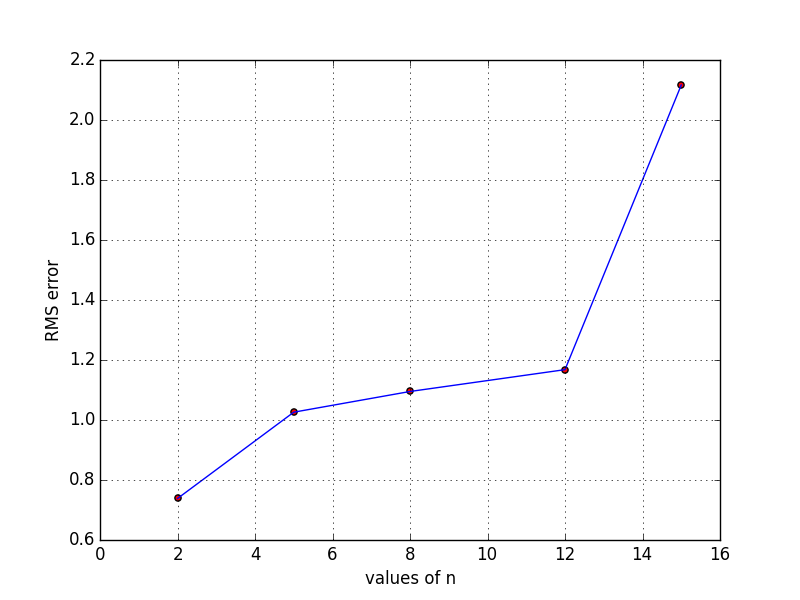
\includegraphics[scale=0.75]{figure_1.png}
    \caption{Plot showing that as n increases the RMS error of the solution of a system of linear equations, with the hilbert matrix values as its coefficients, increases.The red dots show the actual error values}
	\label{fig:err1}
\end{figure}

\begin{table}[ht]
\centering
\label{my-label}
\begin{tabular}{|c|c|c|}
\hline
 \textbf{n}&\textbf{RMS Error}&\textbf{Condition Number}  \\ \hline
 2&0.73833521&15.0167409881  \\ \hline
 5&1.02602254&282901.77002 \\ \hline
 8&1.09505307&7657562245.89 \\ \hline
 12&1.16783884&5.89342127254e+15 \\ \hline
 15&2.11656192&1.74359790918e+17 \\ \hline
\end{tabular}
\caption{Table showing the values of n and the RMS error after solving the system of linear equations with \textbf{hilbert(n)} as the coefficients.}
\end{table}
The table of n and errors appears on page 4.
The corresponding python code can be found at \ref{code:problem2a}

\subsection{Solving system of linear equations with coefficients as hilbert(n) for n=3}
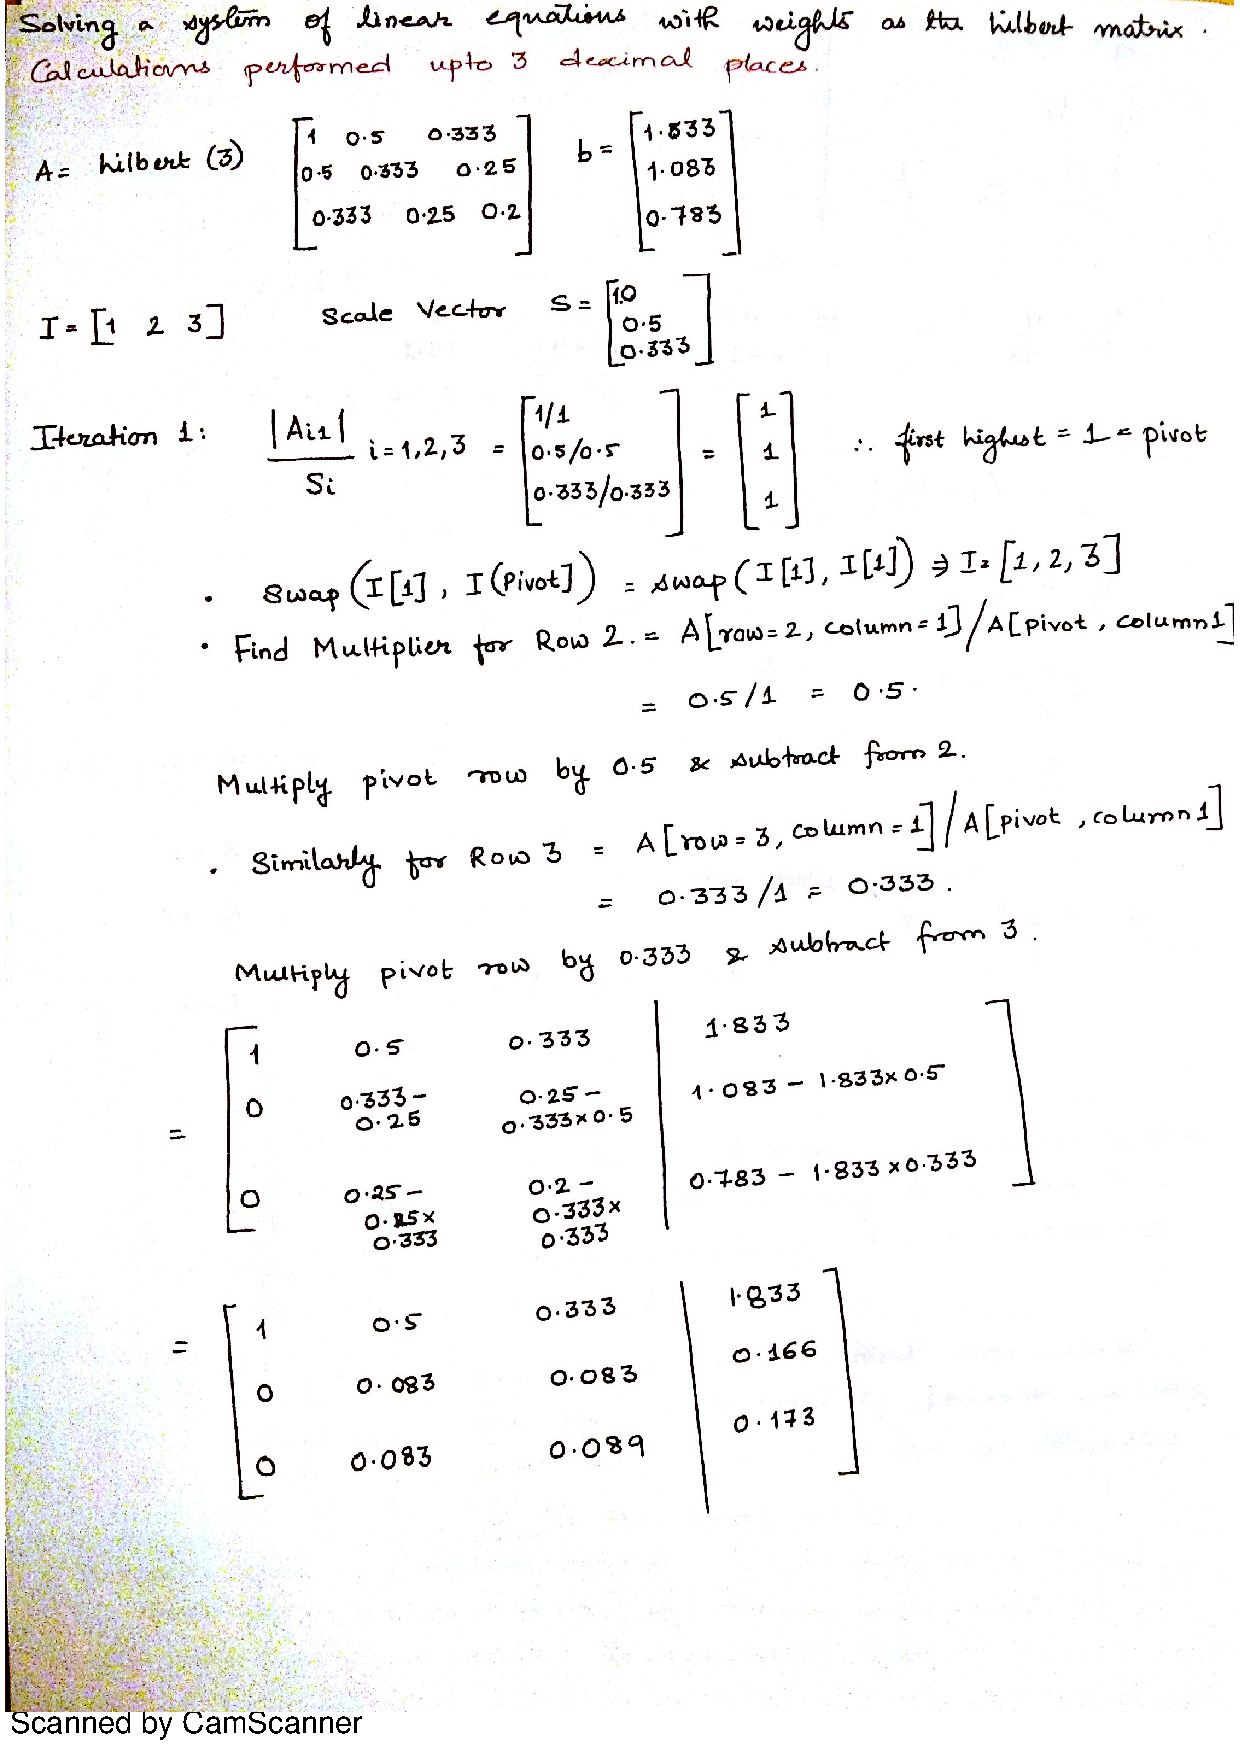
\includepdf[pages=-]{NewDoc1.pdf}
\clearpage
\section{Appendix A}\label{code:problem2a}
Python source code for \ref{prob2a}.
{\footnotesize
\begin{lstlisting}


from __future__ import division
from scipy.linalg import hilbert
import numpy as np
from pprint import pprint
import pylab as pl

def new_solve(A,b):
    A = np.asarray(A, np.float)
    b = np.asarray(b, np.float)
    # Create the scale vector max(abs(ri)) of each row ri in A
    S = np.zeros(A.shape[0], np.float)
    S = np.max(np.abs(A), axis=1)
    # Create the Index vector
    I = np.asarray(range(np.max(S.shape)))
    # iterate over as many times as there are rows (r = 0 to rmax)
    for idx in range(len(I)):
        r = I[idx]
        # get the values from the idx(th) column
        rows_we_want = I[idx:]
        corresponding_column_values = A[rows_we_want, idx]
        # divide the column values by their corresponding scale and get the index of the row with max value
        div_val = np.true_divide(np.abs(corresponding_column_values),S[rows_we_want])
        I_idx = np.argmax(div_val)  
        # because the above index is in I, the actual row is
        act_idx = I[idx:][I_idx]
        max_row = A[act_idx,:]
        # swap current Idx with max_row's idx
        # swap the 0th idx and the new max in the sub array of I
        I[idx:][0], I[idx:][I_idx] = I[idx:][I_idx], I[idx:][0]
        # iterate over remaining rows and update them
        for rem_rows in I[idx+1:]:
            # Get the appropriate multiple of the pivot row. to make the remaining row's idx column a zero
            multiplier = np.true_divide(A[rem_rows][idx],max_row[idx])
            A[rem_rows,idx:] -= max_row[idx:] * multiplier
            b[rem_rows] -= b[act_idx] * multiplier
    return I, A, b

def gauss(I, A, b):
    # returns the solutions to x
    x = np.zeros(I.shape)
    # because this is directly used in indexing and
    # max index of x would be len(x) -1
    len_x = len(x)-1
    # reverse I because we go in reverse I order.
    I = I[::-1]
    for count,row in enumerate(I):
        # get the row which we need to evaluate.
        weighted_sum_of_already_computed_x = 0
        for i in range(count):
            # if its the first value, we need to evaluate once.
            # for the second value, we need to evaluate twice and so on.
            col = len_x-i
            weighted_sum_of_already_computed_x += A[row, col] * x[col]
        # len(x)-count-1 because indices from 3 to 0 when len(x) = 4
        x[len_x-count] = (b[row] - weighted_sum_of_already_computed_x) / A[row,len_x-count]
    return x

def error(x,x_actual):
    diff = np.abs(x-x_actual)
    return np.sqrt(np.divide(np.sum(diff ** 2),x.shape))


if __name__ == '__main__':
    errs = []
    errors = []
    n_vals = [2,5,8,12,15]
    for n in n_vals:
        A = hilbert(n)
        b = np.sum(A,axis=1) 
        I,A,b = new_solve(A,b)
        x = gauss(I,A,b)
        errors.append(error(x,b))
        print n,errors[-1]
    pl.plot(n_vals, errors,c='b')
    pl.grid()
    pl.scatter(n_vals, errors,c='r',marker="o")
    pl.xlabel("values of n")
    pl.ylabel("RMS error of partial pivot and actual solution of hilbert(n)")
    pl.show()

\end{lstlisting}
}
\end{document}
